\begin{figure*}[ht]
    \centering
    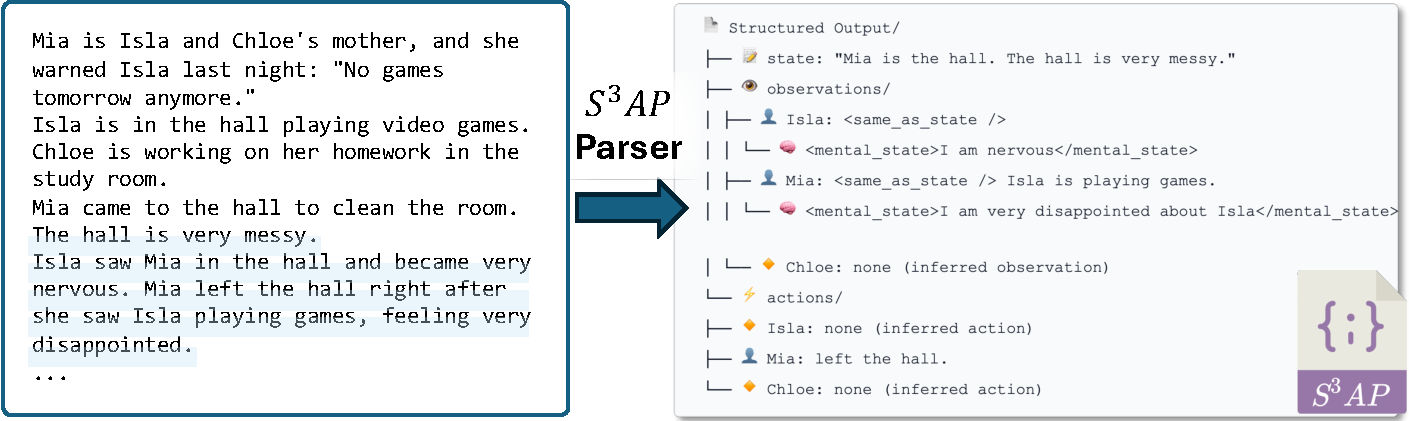
\includegraphics[width=0.9\textwidth]{figs/swm-sap-example-fig3.pdf}
    \caption{An example of free-form narrative parsed into \protocolname. The highlighted text is trasformed to the \protocolname representation with the \texttt{state} field which tracks the overall environment state, \texttt{observations} of each agent and \texttt{actions} of each agent. 
    }
    \label{fig:swm-sap}
\end{figure*}

\section{Social World Model with \protocolname}
\label{sec:protocol}

To overcome the lack of social reasoning in traditional world models \citep{wong2023wordmodelsworldmodels, worldmodels2018david}, we conceptually formalize \textit{social} world models (\S\ref{ssec:swm-formulation}) and introduce a new representation (\protocolname) to power these social world models (\S\ref{ssec:sssap-definition}).


\subsection{Social World Model Formulation}\label{ssec:swm-formulation}

Inspired by $N$-agent Dec-POMDP framework \citep{bernstein2002complexity,nair2003taming}, we formulate a social world
with a state space $\mathcal{S}$, an action space $\mathcal{A}$, an observation space $\mathcal{O}$, a transition function $T: \mathcal{S} \times \mathcal{A} \rightarrow \Delta(\mathcal{S})$, an observation function $\Omega: \mathcal{A} \times \mathcal{S} \rightarrow \Delta(\mathcal{O})$.
For $N$ social agents, we define $\mathcal{A} = \mathcal{A}_1 \times \cdots \times \mathcal{A}_N$ and $\mathcal{O} = \mathcal{O}_1 \times \cdots \times \mathcal{O}_N$ as the joint action and observation spaces.

Rather than restricting the agent to conventional world modeling where observations only capture external states, we redefine the observation space to encompass a rich set of social and psychological factors. Specifically, for each agent $i$, the observation space includes both \textbf{external observations} $\mathcal{O}^{\text{ex}}_i$ and \textbf{introspective observations} $\mathcal{O}^{\text{in}}_i$. The external observations capture information from the environment and other agents, e.g., whether someone exited a room. 
In contrast, the introspective observations include the agent’s internal mentals states, such as their \textit{beliefs}, \textit{goals}, \textit{moral values}, and \textit{emotions}.
Correspondingly, the agent’s action space expands beyond environmental manipulation to include introspective operations such as recalling memories, reflecting on past actions, and updating beliefs. These expansions enable the agent to act not merely reactively but reflectively, a necessary step for modeling complex social behaviors such as empathy, deception, forgiveness, and norm enforcement \citep{shen2024heartfeltnarrativestracingempathy, su2025ailiedarexaminetradeoffutility, forbes2021socialchemistry101learning}.

At time step $t$, each agent $i$ interacts with the social world model by issuing an action $a_i^t$ and receiving an observation $o_i^t$. It then makes decision along with its memory $\mathcal{M}_i^t$ and policy $\pi_i: \mathcal{M}_i^t \times \mathcal{O}_i^t \rightarrow \Delta(\mathcal{A}_i^t)$.
Then a \textbf{social world model} computes:
\begin{align}
   p(\mathcal{A}_t^{-i} \mid \mathcal{S}_t) &\text{;} \\
   p(\mathcal{S}_{t+1} \mid \mathcal{S}_{t}, \mathcal{A}_t^{-i}, a_t^i) &
\end{align}

Equation (1) predicts other agents’ actions from the social world state, and Equation (2) updates the state given all agents’ actions.
Unlike traditional world models, which model passive physical transitions \citep{worldmodels2018david, worldmodels2023xiang, xiang2024pandorageneralworldmodel}, this formulation considers other active agents as part of the social world.

\subsection{\protocolname: Social World State Representation}\label{ssec:sssap-definition}
Building on this formulation, we introduce an \textbf{LLM-powered general-purpose structured representation of social world states}, motivated by the limitations of using raw free-form text alone for social world modeling.
Specifically, we propose a protocol to encode such social narratives into a structured representation (i.e., \protocolname).
As shown in Figure \ref{fig:swm-sap}, given a free-text narrative describing a social interaction at time $t$,  \protocolname-parser parses the narrative into a structured representation of a sequence of descriptions for the environment, agents' observations and actions.
We could use either free-form text or special symbols to describe environment state, agents' observations and actions.
For example, \texttt{<same\_as\_state>} indicates that the agent’s observation is identical to the full environment state.
These symbols can be customized and extended to support more complex social interactions for more efficient characterization of $\mathcal{S}^t$.

Under the configuration of \protocolname, we can encode free-text narratives into a structured representation.
This representation serves as an operationalization of the social world state $\mathcal{S}^t$ at time step $t$ defined above, up to the information present (or inferable) in the narrative.
Given a \protocolname representation of a state of the social world $\mathcal{S}^t$, a social world model could be a generative model that takes agent's actions as input and outputs the next environment state, agents' observations, and other agents' next actions.

Inducing a social world model in this way offers unique advantages:
(1) the protocol provides better structure than pure text narratives with both symbolic and free-form text, enabling more systematic social reasoning (\S \ref{sec:social_understanding}).
(2) By framing the task as predicting \protocolname representation, we can harness the power of LLMs to make the configuration of social world models more efficient and scalable (\S \ref{sec:building_swm}).

